%% LyX 2.0.3 created this file.  For more info, see http://www.lyx.org/.
%% Do not edit unless you really know what you are doing.
\documentclass[12pt,english]{article}
\usepackage[latin9]{inputenc}
%\setlength{\headheight}{15pt}
%\usepackage{fancyhdr}
%\pagestyle{p}
\setcounter{secnumdepth}{3}
\setcounter{tocdepth}{3}
\usepackage{mathtools}
\usepackage{amssymb}
\usepackage{dot2texi}
\usepackage{listings}
\usepackage{tikz}
\usepackage{graphicx}
\usepackage{setspace}
\onehalfspacing
\usepackage[unicode=false,pdfusetitle,
 bookmarks=true,bookmarksnumbered=true,bookmarksopen=false,
 breaklinks=false,pdfborder={0 0 0},backref=false,colorlinks=false]
 {hyperref}

\usepackage{color}

\definecolor{mygreen}{rgb}{0,0.6,0}
\definecolor{mygray}{rgb}{0.5,0.5,0.5}
\definecolor{mymauve}{rgb}{0.58,0,0.82}
\lstset{
backgroundcolor=\color{white},   % choose the background color; you must add \usepackage{color} or \usepackage{xcolor}
  basicstyle=\footnotesize,        % the size of the fonts that are used for the code
  breakatwhitespace=false,         % sets if automatic breaks should only happen at whitespace
  breaklines=true,                 % sets automatic line breaking
  captionpos=b,                    % sets the caption-position to bottom
  commentstyle=\color{mygreen},    % comment style
  deletekeywords={...},            % if you want to delete keywords from the given language
  escapeinside={\%*}{*)},          % if you want to add LaTeX within your code
  extendedchars=true,              % lets you use non-ASCII characters; for 8-bits encodings only, does not work with UTF-8
  frame=single,                    % adds a frame around the code
  keywordstyle=\color{blue},       % keyword style
  language=C,                      % the language of the code
  morekeywords={*,...},            % if you want to add more keywords to the set
  numbers=left,                    % where to put the line-numbers; possible values are (none, left, right)
  numbersep=5pt,                   % how far the line-numbers are from the code
  numberstyle=\tiny\color{mygray}, % the style that is used for the line-numbers
  rulecolor=\color{black},         % if not set, the frame-color may be changed on line-breaks within not-black text (e.g. comments (green here))
  showspaces=false,                % show spaces everywhere adding particular underscores; it overrides 'showstringspaces'
  showstringspaces=false,          % underline spaces within strings only
  showtabs=false,                  % show tabs within strings adding particular underscores
  stepnumber=1,                    % the step between two line-numbers. If it's 1, each line will be numbered
  stringstyle=\color{mymauve},     % string literal style
  tabsize=2,                       % sets default tabsize to 2 spaces
  title=\lstname                   % show the filename of files included with \lstinputlisting; also try caption instead of title
}

\makeatletter
%%%%%%%%%%%%%%%%%%%%%%%%%%%%%% User specified LaTeX commands.
\usepackage[english]{babel}
\newcommand{\BigO}[1]{\ensuremath{\operatorname{O}\bigl(#1\bigr)}}


\makeatother

\begin{document}

\title{Implemention of Reverse Time Migration on FPGA}
\author{Conghui He}

\maketitle

\tableofcontents
%include the introduction
% vim:ts=4:sw=4
%
% Copyright (c) 2008-2009 solvethis
% Copyright (c) 2010-2012 Casper Ti. Vector
% Public domain.

\specialchap{绪言}

本文档是“北京大学论文文档模版”的说明文档,
同时也是使用模版的一个示例。

pkuthss 文档模版由三部分构成:
\begin{itemize}
	\item \textbf{pkuthss 文档类}:
		其中进行了学位论文所需要的一些基本的设定,
		主要包括对基本排版格式的设定和提供设置论文信息的命令。
	\item \textbf{pkuthss-extra 宏包}:
		其中实现了学位论文中用户可能较多用到的一些额外功能,
		例如自动在目录中加入参考文献和索引的条目和%
		自动根据用户设定的文档信息对所生成 pdf 的作者、标题等属性进行设置等。
	\item \textbf{说明(示例)文档}:
		说明文档即本文档,
		在安装(见第 \ref{sec:inst} 节)之后应该可以用 \TeX{} 系统提供的
		\verb|texdoc| 命令调出:
\begin{Verbatim}[frame=single]
texdoc pkuthss
\end{Verbatim}
		同时,
		本文档的源代码(位和本文档的 pdf 文件处于同一目录下)%
		也正是用户撰写自己的学位论文时的一个模版:
		用户只需按照模版中的框架修改代码,
		即可写出自己的论文。
\end{itemize}

在此之前,包括 dypang\supercite{dypang}、FerretL\supercite{FerretL}、%
lwolf\supercite{lwolf}、Langpku\supercite{Langpku}、%
solvethis\supercite{solvethis} 等的数位网友均做过学位论文模版的工作。
本论文模版是 solvethis 的 pkuthss 模版的更新版本,
更新的重点是重构和对新文档类、宏包的支持。

pkuthss 文档模版现在的维护者是 Casper Ti. Vector\footnote%
{\href{mailto:CasperVector@gmail.com}{\texttt{CasperVector@gmail.com}}}。%
pkuthss 文档模版目前托管在 Google Code 上,
其项目主页是:\\
\hspace*{\parindent}\url{http://code.google.com/p/caspervector/}


%% vim:ts=4:sw=4
%
% Copyright (c) 2008-2009 solvethis
% Copyright (c) 2010-2012 Casper Ti. Vector
% Public domain.

\specialchap{绪言}

本文档是“北京大学论文文档模版”的说明文档,
同时也是使用模版的一个示例。

pkuthss 文档模版由三部分构成:
\begin{itemize}
	\item \textbf{pkuthss 文档类}:
		其中进行了学位论文所需要的一些基本的设定,
		主要包括对基本排版格式的设定和提供设置论文信息的命令。
	\item \textbf{pkuthss-extra 宏包}:
		其中实现了学位论文中用户可能较多用到的一些额外功能,
		例如自动在目录中加入参考文献和索引的条目和%
		自动根据用户设定的文档信息对所生成 pdf 的作者、标题等属性进行设置等。
	\item \textbf{说明(示例)文档}:
		说明文档即本文档,
		在安装(见第 \ref{sec:inst} 节)之后应该可以用 \TeX{} 系统提供的
		\verb|texdoc| 命令调出:
\begin{Verbatim}[frame=single]
texdoc pkuthss
\end{Verbatim}
		同时,
		本文档的源代码(位和本文档的 pdf 文件处于同一目录下)%
		也正是用户撰写自己的学位论文时的一个模版:
		用户只需按照模版中的框架修改代码,
		即可写出自己的论文。
\end{itemize}

在此之前,包括 dypang\supercite{dypang}、FerretL\supercite{FerretL}、%
lwolf\supercite{lwolf}、Langpku\supercite{Langpku}、%
solvethis\supercite{solvethis} 等的数位网友均做过学位论文模版的工作。
本论文模版是 solvethis 的 pkuthss 模版的更新版本,
更新的重点是重构和对新文档类、宏包的支持。

pkuthss 文档模版现在的维护者是 Casper Ti. Vector\footnote%
{\href{mailto:CasperVector@gmail.com}{\texttt{CasperVector@gmail.com}}}。%
pkuthss 文档模版目前托管在 Google Code 上,
其项目主页是:\\
\hspace*{\parindent}\url{http://code.google.com/p/caspervector/}



\section{Field Programmable Gate Array}

\subsection{An Overview of FPGA}
Field Programmable Gate Array (FPGA) is a type of integrated circuit (IC)
containing a matrix of logic cells that can be programmed by a user to act
as an arbitrary integrated circuit.

The first field programmable gate array is manufactured by Xilinx
in 1985. However, compared with the widespread of computers, FPGA
was primarily made use of in telecommunications and networking in
the 1990s due to both the sophistication and the volume of the production.

Using the pre-built logic blocks and
programmable routing resources, you can configure these chips to implement
custom hardware functionality in high performance. For example, one can implement a
interrupt controller, a digital filter or even a processor on the basic of
FPGA.

In the past, FPGA technology could be used only by
engineers with a deep understanding of digital hardware design. Thus FPGA is
not as widely use as general purpose processor around the world. But in
the recent years, some companies encapsulated the underlining details of
FPGA and rised several suits of development tools kits to provide a higher
abstract interface for develops. The developers who designing the FPGA now
just need to task in the software and compile them down to a configuration
file or bitstream that contains information on how to components should be
wired together, which makes the task much easier and more and more
developers devotes their energies to FPGA.

\subsection{The Architecture of FPGA}

A typical layout of FPGA (see Figure~\ref{fig:fpga_arch}) is an array of
interconnected programmable logic blocks or configurable logic blocks. It
provides the designer with programmable logic blocks that contain the pool
of combinatorial blocks and flip-flops to be used in the design. Logic is
often used in conjunction with memory. Clock conditioning has also become
commonplace, and support in the form of Delay Locked Loops (DLLs). Phase
Locked Loops (PLLs) is also provided inside the same silicon chip. Finally,
an FPGA chip does not lead a solitary life isolated from the rest of the
world. It needs to be easily interfaced to other chips or external signals.
In order to make this interfacing easier, FPGA vendors have invested a
great deal of effort in enhancing the flexibility of the input/output
blocks behind the chip pads. Each pad can serve as an input, an output, or
both. The list of electrical standards supported is extensive, and novel
techniques for maximizing bandwidth, such as clocking data in using both
edges of the clock, are widely supported~\cite{fpgaintro}.

\begin{figure}
  \centering
  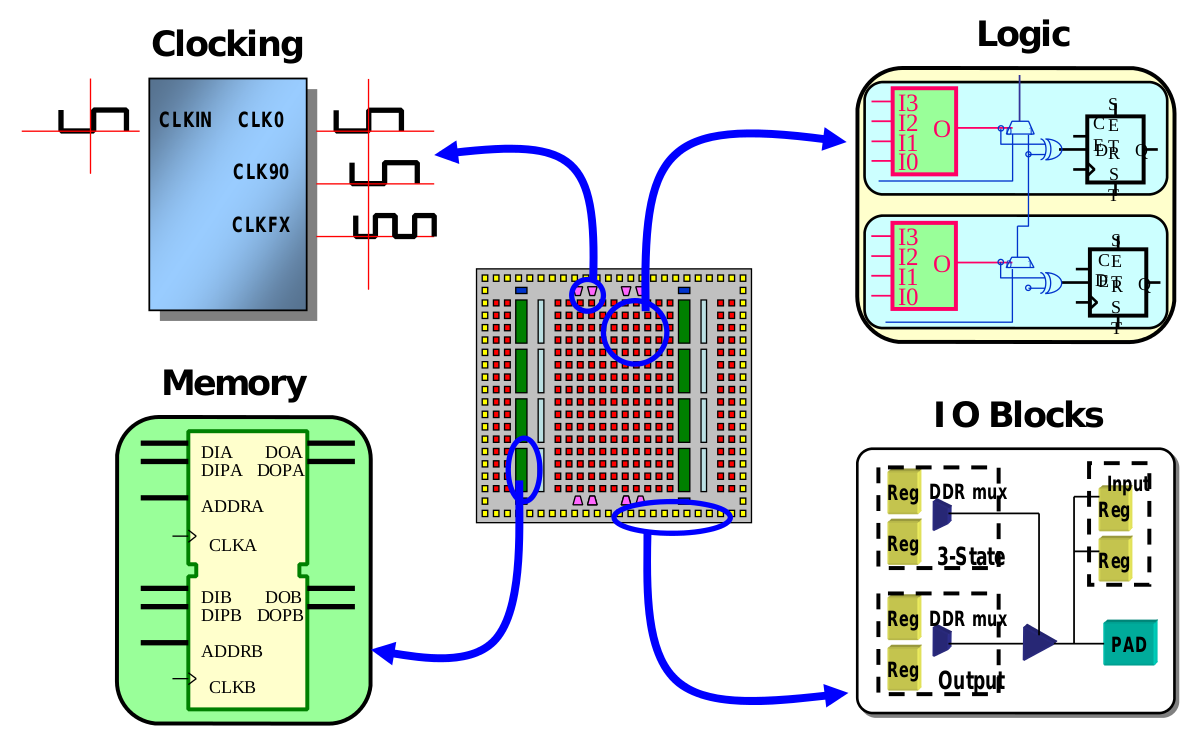
\includegraphics[scale=0.25]{img/fpga_arch.png}
  \caption{Typical structure of modern FPGA}
  \label{fig:fpga_arch}
\end{figure}

Xilinx is the largest vendors of modern FPGA , their latest product, such
as Spartan-3 generation, general consist of five fundamental programmable
functional elements, configurable Logic Blocks (CLBs), Input/Output Blocks
(IOBs), BLOCK RAM, Multiplier Blocks, and Digital Clock Manager (DCM).

\begin{itemize}

  \item \emph{Configurable Logic Blocks (CLBs)} contain flexible Look-Up
    Tables (LUTs) that implement logic plus storage elements used as
    flip-flops or latches. CLBs perform a wide variety of logical functions
    as well as store data.

  \item \emph{Input/Output Blocks (IOBs)} control the flow of data between
    the I/O
    pins and the internal logic of the device. IOBs support bidirectional
    data flow plus 3-state operation. Supports a variety of signal
    standards, including several high-performance differential standards.
    Double Data-Rate (DDR) registers are included.

  \item \emph{Block RAM} provides data storage in the form of 18-Kbit
    dual-port
    blocks.

  \item \emph{Multiplier Blocks} accept two 18-bit binary numbers as inputs
    and
    calculate the product. The Spartan-3A DSP platform includes special DSP
    multiply-accumulate blocks.

  \item \emph{Digital Clock Manager (DCM)} Blocks provide self-calibrating,
    fully
    digital solutions for distributing, delaying, multiplying, dividing,
    and phase-shifting clock signals.
\end{itemize}

These elements are organized as shown in Figure~\ref{fig:spartan_arch},
using the Spartan-3A FPGA
array as an example. A dual ring of staggered IOBs surrounds a regular
array of CLBs in the Spartan-3 and Extended Spartan-3A family. The
Spartan-3E family has a single ring of inline IOBs. Each block RAM column
consists of several 18-Kbit RAM blocks. Each block RAM is associated with a
dedicated multiplier. The DCMs are positioned with two at the top and two
at the bottom of the device, plus additional DCMs on the sides for the
larger devices.

\begin{figure}[h]
  \centering
  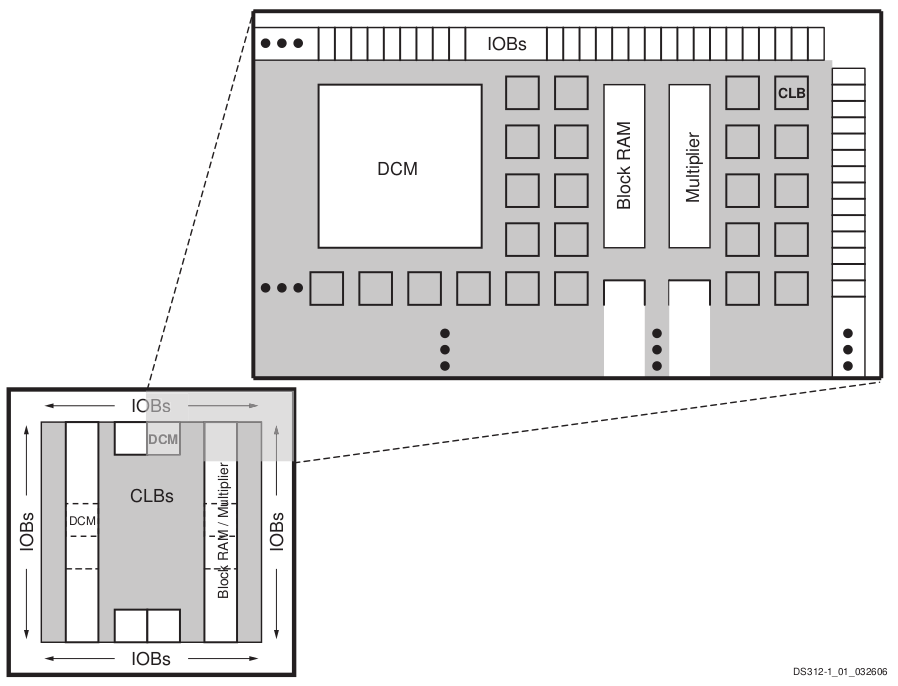
\includegraphics[scale=0.3]{img/spartan_arch.png}
  \caption{Spartan-3A Platform Architecture}
  \label{fig:spartan_arch}
\end{figure}

The Spartan-3 generation features a rich network of traces that
interconnect all five functional elements, transmitting signals among them.
Each functional element has an associated switch matrix that permits
multiple connections to the routing\cite{fpgaug}.

\subsection{Designing FPGA with Maxcompiler}

The usual way to design FPGAs is to write a behavioral model in
a Hardware Description Language (HDL), like Verilog or VHDL, which
supports concurrency and synchronous circuits. Concurrency allows
you to create fully parallel, independent processes, each describing
how to update some variables continuously. Synchronous circuits, instead,
are those made of flip-flops that change their state only on the edge
of some clock signal.

After the design has been written and verified with an HDL simulator,
a compiler creates a list of all the logic gates and the wires (nets)
that must connect them to reproduce the functionality of the HDL model.
After this logic synthesis, layout programs read the netlist and several
constraints files to find out which logic gates inside the FPGAs must
be used and which physical, internal wires must connect them to each
other. The end result is the bit file that the FPGA reads at power-up.

The above kind of FPGA configuring developing is still an obstruct for
those who seldom care much about hardware or digital circuit. In order to
make full use of FPGA, Maxeler Inc, develops a compiler where software
engineer can perform configuring developing with their daily used
developing language, such as C, and Java.

\subsubsection{Maxeler Acceleration Technology}

\emph{Maxcompiler} is a commercial product that is manufactured by Maxeler.
It is a compiler system for Maxeler hardware acceleration solutions using
FPGAs. The compiler system is a good assistant for software engineering
developer to create FPGA configuring because it has a higher abstract of
the underlining subtle hardware information, and then provide a set of
Application Interface for developers.

Figure~\ref{fig:maxeler_acceleration_system} have a sketch of Maxeler
acceleration system architecture. The system comprises several FPGAs
attached directly to the local memory and to a host CPU via PCI Express.

\begin{figure}
  \centering
  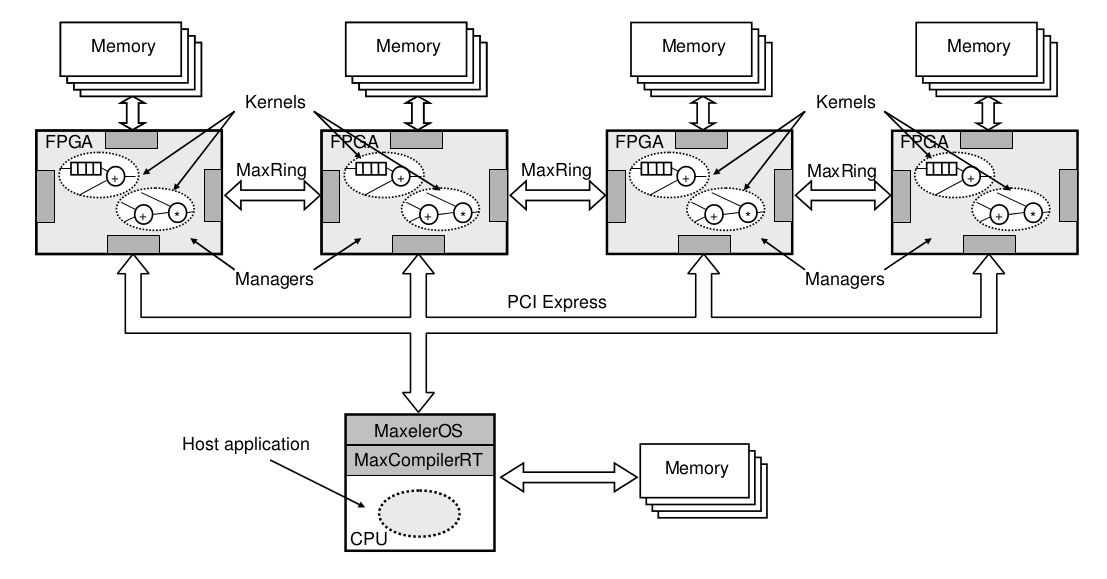
\includegraphics[scale=0.35]{img/overview_of_maxeler_acceleration_system.png}
  \caption{An overview of Maxeler acceleration system}
  \label{fig:maxeler_acceleration_system}
\end{figure}

While developing the application, develops identify the runtime intensive part
and tunning them into FPGA configuration, which is called \emph{kernel} and
\emph{manager} in the acceleration system. After all the configured FPGA
files are compiled and downloaded into FPGA EEPROM, the host (CPU) code
communicate with FPGA with the help of \emph{Maxeler OS}. The Maxeler OS
provide a set of API called \emph{MaxCompierRT}, a runtime library to load
the configuration to FPGA and transfer data from/to FPGA.

The programming paradigm of FPGA designing is different from the general
programming paradigm, such as C/C++. The FPGA gains it high efficiency from
the parallel working of the different Configurable Logic Block (CLB). The
program describes the computations structurally (in space) rather than
specifying the sequence of processor instructions (in
time)\cite{max_white_paper}.

\subsubsection{Development Flow}
If the developer want to accelerate an application after he identifies the
runtime intensive part of the program, what he needs includes three parts,
designing the kernel, manager configuration and adapt the host application.
All the three parts can be easily implemented with the help of Maxeler
compiler tools. Figure \ref{fig:development_flow} presents the development flow with the main
components of MaxCompiler.

\begin{figure}[h]
  \centering
  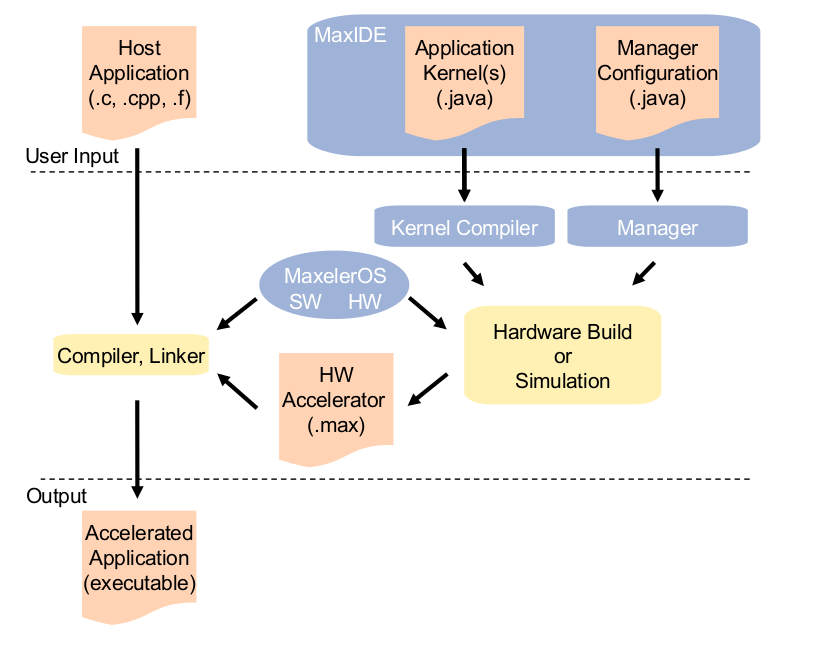
\includegraphics[scale=0.4]{img/development_flow.png}
  \caption{Maxeler development flow}
  \label{fig:development_flow}
\end{figure}

The first stage, designing the kernel, is the most critical part of the
acceleration. Kernel has the similar meaning with that in CUDA GPU
programming, which refers to the most computationally-demanding part that
should be executed in the FPGA/GPU board. Java, the well-known high level
language is used to develop the kernel. Here we just the syntax of Java,
excluding the massive Java library. In addition, the Maxeler provides a set
of library that use to configure the kernel with the help of the
MaxCompiler. Instead of using the phase ``programming to configure kernel
with Java'', it is more appropriate to say ``designing the configure kernel
with Java'', because paradigm of designing the FPGA application with
MaxCompiler is to describe the structure of the logic, rather than telling
the FPGA the sequence of the process instructions, which we use in the
general purpose programming.

When the kernel is well configured, we need to set up a manager for it. The
manager is responsible for how to set up the kernel, for example, pass the
parameter to kernel that kernel expects. What's more, the manager is also
responsible to cooperate the kernels together if there are multiple
kernels, or multiple FPGA boards working for the same problem. The manager
can configure the kernel for simulation or for real work kernel.
Configuring the kernel for simulation is preferred because it saves time to
generate it. A full hardware build may take you hours or even weeks
depending on the complexity of the kernel.

Whenever the simulation kernel or the hardware kernel is build, it is
possible to linked it with the host application. Maxeler provides a set of
runtime library in C/C++ and Fortran to help the programmer to develop. The
communication between the local machine and FPGA device is via the runtime
library and interface, which could help the developer to transform data
from/to the FPGA Device.

The MaxCompiler can link them together in the last stage of the compilation
and generate the ordinary binary executable file.

\subsection{Advantage of FPGA Designing}

FPGA chip adoption across all industries is driven by the fact that FPGAs
combine the best parts of ASICs and processor-based systems. FPGAs provide
hardware-timed speed and reliability, but they do not require high volumes
to justify the large upfront expense of custom ASIC design. Reprogrammable
silicon also has the same flexibility of software running on a
processor-based system, but it is not limited by the number of processing
cores available.

Unlike processors, FPGAs are truly parallel in nature, so
different processing operations do not have to compete for the same
resources. Each independent processing task is assigned to a dedicated
section of the chip, and can function autonomously without any influence
from other logic blocks. As a result, the performance of one part of the
application is not affected when you add more processing.

In addition, FPGAs are blurring the lines between hardware and software in systems.
FPGA devices are inherently soft-programmable and may be changed
dynamically during the operation of a system. More compellingly, FPGA devices
now also contain embedded microprocessors within the logic fabric,
and these microprocessors can run Linux. Imagine a Linux computer
with up to millions of gates of flexible logic immediately around
it. One way to grok this new paradigm is to think of the following:
Software is configuration bits for hardware.


\chapter{Reverse Time Migration Algorithm}

The purpose of the \emph{seismic exploration} is to understand the
constitution of the interior earth as much as possible. As we know, it is
impractical or even impossible to penetrate the earth and put your camera
there to capture the image, other indirect approaches are used to attain
the similar or same result. These approaches includes seismological
measurement, electromagnetic measurement and gravity measurement. As these
approaches are indirect, they usually give a analyze or indication of the
measured result. Some tools, such as computers, are required as part of the
analyze and the capability of the tools may be the bottleneck of the
analyze. For example, in the past, with the poor computational performance
of the computer, the data in only a small region and in a low resolution
could the seismologists analyzed due to the limited computing power.

As the Moore's Law indicates that the number of transistors double every 18
months, the computer gains much more computing power than before. Some
seismological method, which are computationally-demanding, seems not
practical in the past, can be implemented by utilizing the advanced
technology today. One of the most useful but computationally-demanding
algorithm, Reverse Time Migration algorithm, also comes into reality.

Reverse Time Migration is an algorithm of seismic migration. And seismic
migration is one of the most important part of seismic exploration, and
more specifically, seismic imaging. By seismic migration, the constitution
of the interior earth could be imaged, sketching, for example, the water,
rocks, gas, oil, faults etc in the subsurface.

\section{General Process of Seismic Exploration}

Seismic exploration, as one of the background knowledge of this thesis,
is explained in this section. Figure (\ref{fig:sea_floor_seismic}) shows a
typical scenario of a marine
based seismic exploration. The vessel will inject waves periodically by the
air gun. The waves just injected will spread in all direction quickly until
it penetrate different media, such as rocks, ands, gas, or oil beneath the
water, where the waves will reflect back or refract through another medium.
The reflected waves, or those refracts first, then reflected waves would be
recorded by an large array of Geo phones. In figure
(\ref{fig:sea_floor_seismic}), another smaller ship shows up, dragging a
cable
which contains an array of sensors to record the reflected signals.

\begin{figure}
  \centering
  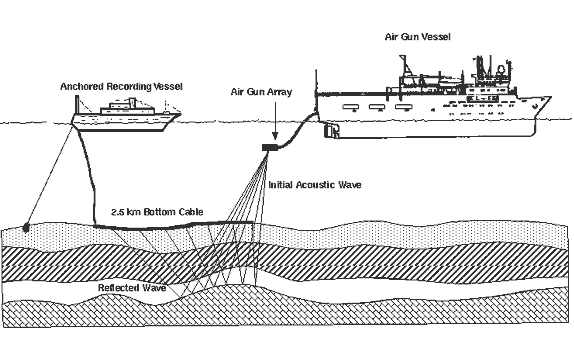
\includegraphics[scale=0.5]{img/Seafloor_Seismic.png}
  \caption{Marine-based Seismic Exploration}
  \label{fig:sea_floor_seismic}
\end{figure}

Geophysics data processing then follows the process of recording the
signals. First of all, multiple steps should be applied to perform the
preprocessing. For example, use the bandpass filter to remove the noise.
And last of all, is the migration step to reconstruct the image of
subsurface.

The detail of how the data are processed is not the topic of this thesis,
so I won't explain it too much. Those who are interested in the subject can
find more information with the help of the search engine. In this thesis, I
only concern about what is relevant with the FPGA implementation of the
computational part, which is explained in next section.

\section{Reverse Time Migration}

In this section, I present a general introduction for Reverse Time
Migration with some seismic terminologies. Revere Time Migration use the
source and recorded signals as input, following a series of computing, then
produce an image of the velocity model, which can maps to the real image of
the interior earth.

You may wonder why the velocity can be mapped to the real constitution of
the interior earth. There are several different objects inside the earth,
such as water, rocks, salt, gas, oil and they are the medium while the wave
propagating through them. The speed of the wave, usually the acoustic wave,
varies from the different medium, for example, the speed of sound is nearly
340 meter per second at temperature 20 degree. If we can generate a model
of the speed inside the earth, we can infer what is inside the earth.

The conventional one-way pre-stack depth migration approach, works well in
the layer medium, shown in Figure (\ref{fig:layer_structure}). If the desired
layer, such as the gas or the oil lies horizontally, it can be easily
discovered with the conventional approach.

\begin{figure}[h]
  \centering
  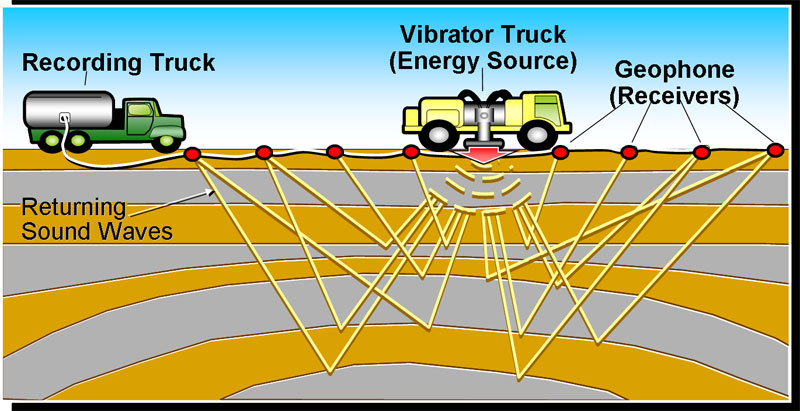
\includegraphics[scale=.45]{img/layer_structure.jpg}
  \caption{Layered structure of the interior earth}
  \label{fig:layer_structure}
\end{figure}

However, not all desired resources are exposed in such a friendly form.
There may be some hill or large rocks beneath the sea, which will obstruct
the desired resource. In addition, some resources will stay in vertical
form or other forms instead of the restrict horizontal form. The
conventional one-way pre-stack depth migration approach could not handle
the previous situation. Thus why Reverse Time Migration emerged.

Reverse Time Migration algorithm is not a new algorithm, instead, it is
first put forward in the 1970s. However, people at that time thinks that it
is impractical or impossible to use such algorithm in practice due to the
tensive  computation requirement. But nowadays, it is impossible to
implement the Reverse Time Migration thanks to the fast developing of
computers.

Instead of just one-way pre-stack depth migration, the Reverse Time
Migration is a two-way pre-stack depth migration, which handles steeply
dipping events, turning waves and multiples. The detail of the algorithm
will be explained in the next section.

Figure (\ref{fig:comparison}) show an introductory example with synthetic
data that illustrates the potential power of the Reverse Time Migration.
There are mainly two part of object in the model, one is water (color from
blue to yellow), the other one is salt (color in red). The figure in the
left is not a real image of the interior earth, but a velocity of that
zone. As the water gets deeper, the speed of the sound becomes faster, so
that is why the color turns from blue to yellow and dark yellow. The salt
is solid object, where the speed of sound is much faster than that in the
water, so the color is in red, a darker color than yellow.

\begin{figure}[h]
  \hfill
  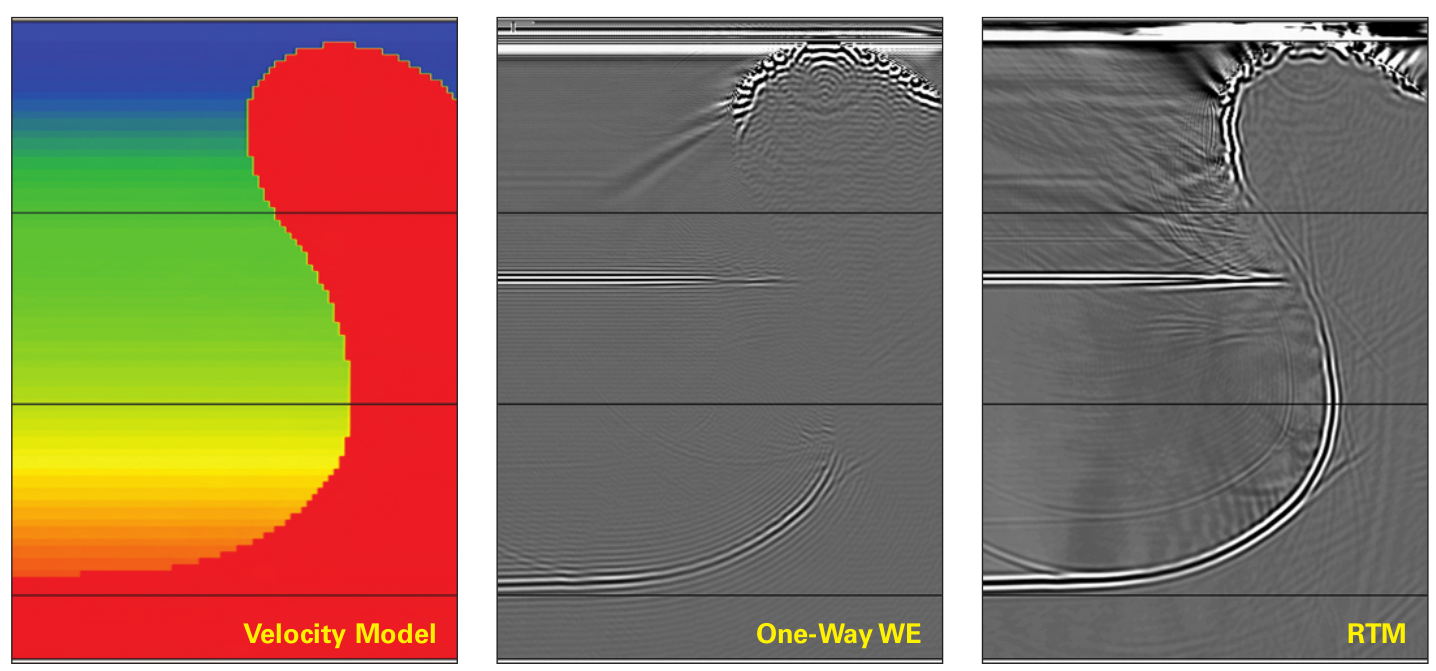
\includegraphics[scale=.25]{img/velocity_model.png}
  \caption{Synthetic comparison of salt flank}
  \label{fig:comparison}
\end{figure}

Concerning about the result, we take a comparison of the middle and right
one in Figure (\ref{fig:comparison}). The middle one is generated using the
one-way wave equation. It is obvious that the salt flank below the overhang
is poorly imaged. On real data, it is difficult to understand the dip and
the structure of sedimentary strata in similar overhang zone. Thus the
potential existence of gas or oil against the salt are impossible to
identify. On the other hand, the last figure, which is produced using the
RTM algorithm, yielding a big improvement. It has a clear profile that is
similar to the original synthetic data.

\section{RTM Algorithm and Analysis}

As it is mentioned in the previous section that the Reverse Time Migration
algorithm can gain a big improvement but it is computationally demanding.
In this section, we have a look at the detail of the algorithm and present
a computation complexity analyze of it.

The main steps of the algorithm is explained as below\cite{rtm}.

\begin{enumerate}
\item the forward extrapolation of a modelled source waved for each shot
  location through a gridded velocity model is performed. And the wave
  field at each time step is saved for later application of the ``imaging
  condition''.
\item the receiver wave field for each shot, which is recorded in the
  field, is backward propagated in time through the same velocity model.
\item at each time step, the corresponding source and receiver wave fields
  are correlated by applying the imaging condition. Thus, the final
  wave field in the source propagating scheme is correlated with the
  initial wave field in the receiver propagation scheme, and so on backward
  through the receiver propagation.
\item the result are summed to form a partial image volume for each shot.
\item the image volumes for consecutive gathers are spatially summed to
  produce the final pre-stack depth image.
\end{enumerate}

So, now you may know why RTM is so computation expensive and has several
decades to be commercially implemented.

\subsection{Mathematical Derivation of RTM}

If we assume that the wave that the wave injects is acoustic wave (sound
wave), then we can use the acoustic wave equation (\ref{eq:acoustic}) as
the first step of the derivation.

\begin{equation}
  \frac{\partial ^2u}{\partial t^2}=c^2 \cdot \left(  \bigtriangledown ^2u \right) +s
  \label{eq:acoustic}
\end{equation}

where \( u = u(x, y, z, t) \) is the pressure field, \(c = c(x, y, z) \) is
the velocity field, \( s = s(x, y, z, t) \) is the source term, and \(
\bigtriangledown ^2 \) is the three dimensional Laplace operator.

The Laplace operator is a second order differential operator in the n-dimensional
Euclidean space, defined as the divergence (\( \bigtriangledown \)) of the gradient
(\( \bigtriangledown f\)). Thus if \( f \) is a twice-differentiable real-valued
function, then the Laplacian of \( f \) is defined by

\[
  \bigtriangleup f = \bigtriangledown ^2 f = \bigtriangledown \cdot
  \bigtriangledown f
\]

Equivalently, the Laplacian of \( f \) is the sum of all the unmixed second
partial derivatives in the Cartesian coordinates:

\[
  \bigtriangleup f = \sum _{i=i} ^n \frac{\partial ^2 f}{\partial x_i ^2}
\]

In particular, if the variable x, y and z denote the three dimensional
Cartesian coordinates, the expansion is:

\begin{equation}
  \bigtriangleup f  = \bigtriangledown ^2 f = \frac{ \partial ^2 f}{\partial x^2} +
                     \frac{ \partial ^2 f}{\partial y^2} +
                     \frac{ \partial ^2 f}{\partial z^2}
  \label{eq:laplacian}
\end{equation}

Thus, replace the Laplacian operator with (\ref{eq:laplacian}), the
equation (\ref{eq:acoustic}) could be derived as:

\begin{equation}
  \frac{\partial ^2u}{\partial t^2}=
  c^2\cdot\left(
  \frac{ \partial ^2 u}{\partial x^2} +
  \frac{ \partial ^2 u}{\partial y^2} +
  \frac{ \partial ^2 u}{\partial z^2}
  \right)
  +s
  \label{eq:acoustic2}
\end{equation}

Equation (\ref{eq:acoustic2}) can be further factored as:
\begin{equation}
  \frac{u_{t+1} - 2u_{t} + u_{t-1}}{dt^2}=
  c^2\left(
  \frac{ \partial ^2 u}{\partial x^2} +
  \frac{ \partial ^2 u}{\partial y^2} +
  \frac{ \partial ^2 u}{\partial z^2}
   \right)
  +s
  \label{eq:acoustic3}
\end{equation}

Then we introduce a method called \emph{stencil}, which is a geometric
arrangement of a nodal group that relate to the point of interest by using
a numerical approximation routine in mathematics, especially the areas of
numerical analysis concentrating on the numerical solution of partial
differential equations. The derivation of stencil from the second order
partial difference is in appendix. Now, equation (\ref{eq:acoustic3}) could
be written as:

\begin{equation}
  \frac{u_{t+1} - 2u_{t} + u_{t-1}}{dt^2}=
  c^2 \cdot\left( \frac{1}{dh^2} \cdot stencil\left( p_t \right) \right)
     +s
  \label{eq:acoustic4}
\end{equation}

where \( dh \) is the distance between the two neighbours of the stencil
operation. For a specific point x, the stencil result of that point in 6th
order is:

\begin{equation}
  \begin{split}
    {f(x)}'' =
    & w_{-3}f\left( x - 3 \Delta x \right) +
      w_{-2}f\left( x - 2 \Delta x \right) +
      w_{-1}f\left( x - \Delta x   \right) + \\
    & w_{0}f\left( x \right) + \\
    & w_{1}f\left( x + \Delta x \right) +
      w_{2}f\left( x + 2 \Delta x \right) +
      w_{3}f\left( x + 3 \Delta x \right)
  \end{split}
\end{equation}

where \( \Delta x \) has the same meaning with \( dh \) in equation
\ref{eq:acoustic4}. To give a better vision, Figure
\ref{fig:6th_order_stencil_1d} give a outline of one dimensional stencil.

\begin{figure}[h]
  \centering
  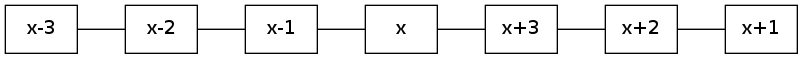
\includegraphics[scale=0.4]{img/6th_order_stencil.png}
  \caption{6th order one dimensional stencil}
  \label{fig:6th_order_stencil_1d}
\end{figure}

Figure (\ref{fig:6th_order_stencil_1d}) give us a array like presentation of
1D stencil, and the result at element i is:

\[
  y\left[ i \right] = c_3  x\left[ i-3 \right] +
                      c_2  x\left[ i-2 \right] +
                      c_1  x\left[ i-1 \right] +
                      c_0  x\left[ i \right] +
                      c_1  x\left[ i+1 \right] +
                      c_2  x\left[ i+2 \right] +
                      c_3  x\left[ i+3 \right];
\]

where \( c_0 \) to \( c_3 \) are dedicated coefficients based on the
different order of the stencil.

In the previous acoustic equation, the stencil is a 6th order 3D stencil,
which is denoted by x, y and z axis. Thus, given a point (x, y, z), there
are 18 (3 x 6) points around and the center point, 19 points altogether,
will be used to perform the calculation. Figure
(\ref{fig:6th_order_stencil_3d}) gives a sketch of such stencil.

\begin{figure}[h]
  \centering
  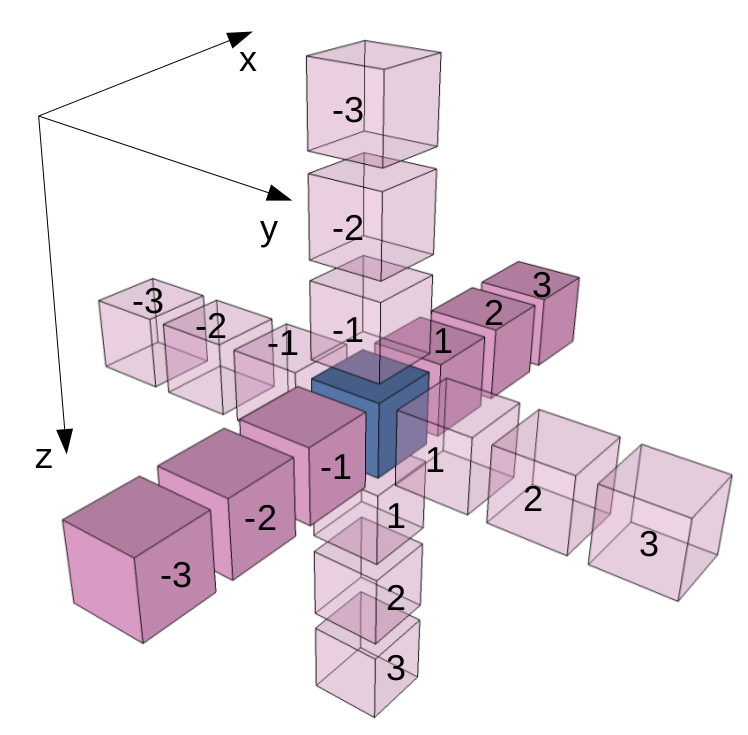
\includegraphics[scale=0.4]{img/stencil_6_3d.png}
  \caption{6th order 3 dimensional stencil}
  \label{fig:6th_order_stencil_3d}
\end{figure}

The calculation of the stencil in Figure (\ref{fig:6th_order_stencil_3d})
is sum of the x, y and z axis. We can draw a formula to denote it.

\begin{equation}
  g(x,y,z) = \sum _{i=-3} ^{+3} w_i  f(i,y,z) +
             \sum _{j=-3} ^{+3} w_j  f(x,j,z) +
             \sum _{k=-3} ^{+3} w_k  f(x,y,k) -
             2f(x,y,z)
 \label{eq:stencil_3d}
\end{equation}

Changing the equation (\ref{eq:stencil_3d}) to the programming psudo-code
is very convenient for programming to code. Listing (\ref{lst:stencil_code_1element})
shows the desired psudo-code.

\begin{figure}
\centering
\lstinputlisting[
  caption={Pseudo code of calculating one element using stencil method},
  label={lst:stencil_code_1element}
  ]
  {code/stencil_1elem.c}
\end{figure}

Listing (\ref{lst:stencil_code_1element}) only works for 1 element in the
array. In practice and in the previous equation (\ref{eq:acoustic}), all
the elements in the three dimension volume should be calculated one by one
except for the boundaries. Thus the complexity of calculating the stencil
in a volume is \BigO{n^3}

Each step of the iteration, what we desire is to calculate the the wave
field of time \( t + 1 \), moving the item \( t \) and \(t-1\) to the right
side of the assignment operator of equation \(\ref{eq:acoustic4}\), we get
the equation (\ref{eq:acoustic5}).

\begin{equation}
  u_{t+1} =
  2u_{t} - u_{t-1} +  dt^2 \left( c^2\cdot\left( \frac{1}{dh^2} \cdot stencil\left( p_t \right) \right)
 +s_t\right)
  \label{eq:acoustic5}
\end{equation}

Now, it is easy to write the pseudo code of coressponding to the equaltion
(\ref{eq:acoustic5}). Storing the wave field in a 4 dimensional array,
including t, x, y, and z dimension. s is also a one dimensional array
storing the the source signal. The psedo code is shown in Listing
(\ref{lst:acoustic}) in page \pageref{lst:acoustic}.

\begin{figure}
  \centering
  \lstinputlisting[
    caption={Pseudo code of calculating forward acoustic wave equation},
    label={lst:acoustic}
  ]
  {code/acoustic.c}
\end{figure}

As you can see, the array u is a four dimensional array. If the nz = ny =
nx = 512, and nt = 500, the size of the array is \( 512^3 * 500 * 4 =
268435456000 \) bytes, that is 250G, which is impossible to store in the
memory. However, the size of the array is much smaller than that in the
reality, because assuming that dt = 0.002, nt = 500, dh = 20, it is recorded for
only 1 second of sound for the cude of 10240m * 10240m * 10240m, nearly a
cube of 10km for a single shot.

What's worse, the algorithm listed in Listing (\ref{lst:acoustic}) is only
part of the RTM algorithm. The Reverse Time Migration algorithm is a
two-way pre-stack depth migration, which is explained in the previous
section, the wave propagation of the source and receiver should be
correlated, to gain the resulting image. The pseudo code\cite{fu11} is shown in
Listing (\ref{lst:rtm}) in page \pageref{lst:rtm}.

\begin{figure}[h]
  \centering
  \lstinputlisting[
    caption={Pseudo code of the RTM algorithm},
    label={lst:rtm}
  ]{code/rtm.c}
\end{figure}

\subsection{Complexity analyze}

Dablain (1986) effectively applies explicit high-order finite
difference spatial derivatives to the acoustic wave equation.
We also apply high-order spatial derivatives to the acoustic
wave equation. Using the \( 2^{nd} \) in space finite differences, the
forward and backward wave field propagations can be calculated as
\cite{rtm_psdm}:

\begin{equation}
  u ^{l(+/-)1} _{i,j,k} = 2u^l _{i,j,k} - u^{l(+/-)1} _{i,j,k} + \Delta t^2
  c^2 _{i,j,k} (\left( \bigtriangledown ^2 u ^l _{i,j,k}  \right) ^ n_0 +
  s ^l _{i,j,k})
\end{equation}

where

\[u^l _{i,j,k} = u(i\Delta x, j \Delta y, k \Delta z, l \Delta t),\]
\[ s^l _{i,j,k} = s(i\Delta x, j \Delta y, k \Delta z, l \Delta t),\]
\[ c_{i,j,k} = u(i\Delta x, j \Delta y, k \Delta z), \]

and \( \Delta t \) =  the temporal step size for finite differencing, \(
\Delta x \), \( \Delta y \), and \( \Delta z \) are the spatial sampling
intervals, and \( \bigtriangledown ^2 u^t _{x, y, z} \) the Laplacian
calculated with \( n^{th} \) order of accuracy at each time step t,
centered at an x-, y-, and z- location. During the backward extrapolation
the source
term is replaced by the recorded input data. The Laplacian with
\( n^{th} _0 \) order accuracy can be given by ().

\begin{equation}
  (\bigtriangledown ^2 u ^l _{i,j,k})^n_0 = w_0(\frac{1}{\Delta x^2} +
  \frac{1}{\Delta y^2} + \frac{1}{\Delta z^2})u^l _{i, j, k} + \Phi
\end{equation}

where

\begin{equation}
  \begin{split}
    \frac{\Phi}{\sum_{m=1} ^{n_0 / 2}w_m} =
      &\frac{1}{\Delta x^2}\left(u^l _{i-m, j, k}+ u ^l _{i+m, j, k}
      \right) + \\
      &\frac{1}{\Delta y^2}\left(u^l _{i, j-m, k}+ u ^l _{i, j+m, k}
      \right) + \\
      &\frac{1}{\Delta x^2}\left(u^l _{i, j, k-m}+ u ^l _{i, j, k+m} \right)
  \end{split}
\end{equation}

where w are finite differencing coefficients of the desire
accuracy. Coefficients are calculated via a series expansion
method. For example, if a second derivative of a function
\( f(x) \) is required to be approximated with \( 6^{th} \) order accuracy
on a uniform grid, the approximation can be written as:

\begin{equation}
  \begin{split}
    {f(x)}'' =
    & w_{-3}f\left( x - 3 \Delta x \right) +
      w_{-2}f\left( x - 2 \Delta x \right) +
      w_{-1}f\left( x - \Delta x   \right) + \\
    & w_{0}f\left( x \right) + \\
    & w_{1}f\left( x + \Delta x \right) +
      w_{2}f\left( x + 2 \Delta x \right) +
      w_{3}f\left( x + 3 \Delta x \right)
  \end{split}
  \label{eq:finite}
\end{equation}

Finite difference weights in (\ref{eq:finite}) can be calcuated using a
series expansion method. The coefficients are symmetrical around \( w_0 \)
for a uniform grid.

The cost of the method is approximately given by the following equation:

\begin{equation}
  C_e \approx 2n_t n_x n_y n_z \left( 3n_0 + 19 \right)
  \label{eq:complexity}
\end{equation}

Where \( C_e \) is the number of floating point operations; \( n_t \) is
the number of time steps; \( n_x , n_y , n_z \) are the number of samples
in the x, y and z directions.

So equation (\ref{eq:complexity}) is similar for the algorithm in Listing
(\ref{lst:rtm}) in page \pageref{lst:rtm} for only a single shot. Adding
the number of shots to the complexity, equation (\ref{eq:complexity})
become (\ref{eq:complexity2}).

\begin{equation}
  C_e \approx 2n_s n_t n_x n_y n_z \left( 3n_0 + 19 \right)
  \label{eq:complexity2}
\end{equation}

It is almost unable to calculate such a algorithm in general purpose 
computer in a short time. What's more, the memory can not satisfy the 
requirement. The size of cache in the general purpose computer or some advanced 
server is usually several mega bytes. It is rather small compared with the 
size of the wave field array. The use of cache doesn't gain much in this 
application.


%% The following contains your structure of your thesis and your
%% contribution, comparison with CPU version.


% include the bibliography
\begin{thebibliography}{9}
  \bibitem{fu11} H. Fu and R. G. Clapp, \emph{Eliminating the memory
    bottleneck: an FPGA-based solution for 3d reverse time migration,}
    in Proceedings of the 19th ACM/SIGDA international symposium on Field
    programmable gate arrays, 2011, pp. 65-74.

  \bibitem{herb11} Herb Sutter, \emph{The Free Lunch Is Over: A Fundamental
    Turn Toward Concurrency in Software,} Dr. Dobb's Journal, 30(3), March
    2005. Retrieved 21 November 2011.

  \bibitem{yoon03} K. Yoon, C.Chin, S. Suh, L. Lines, and S. Hong.
    \emph{3D Reverse-time Migration Using the Acoustic Wave Equation:
    An Experience with the SEG/EAGE Data Set.} The Leading Edge, 22(1):38-41,
    2003.

  \bibitem{moore}
    \emph{Moores law, Wikipedia, the free encyclopedia} [online],
    http://en.wikipedia.org/wiki/Moore's\_law.

  \bibitem{shafiq} M. Shafiq, M. Pericas, N. Navarro, and E. Ayguade,
    \emph{A Streaming Based High Performance FPGA Core for 3D Reverse
    Time Migration.}

  \bibitem{river} G. Rivera and C. Tseng.
    \emph{Tiling Optimizations for 3D Scientific Computations.}
    In Proc. Supercomputing, 2000.

  \bibitem{navarro} M. Shafiq, M. Pericas, R. de la Cruz, M. Araya-Polo,
    N. Navarro, and E. Ayguade.
    \emph{Exploiting Memory
    Customization in FPGA for 3D Stencil Computations.}
    In Proc. International Conference on Field
    Programmable Technology (FPT), pages 38-45, 2009.

  \bibitem{garey} W. Spotz and G. Carey.
    \emph{A High-Order Compact Formulation for the 3D Poisson Equation.}
    Numerical Methods for Partial Differential Equations, 1996.

  \bibitem{top500}
    \emph{Top500 super computer sites - November 2012} [online],
    http://www.top500.org

  \bibitem{chin}K. Yoon, C.Chin, S. Suh, L. Lines, and S. Hong.
    \emph{3D Reverse-time Migration Using the Acoustic Wave
      Equation: An Experience with the SEG/EAGE Data
    Set. }
    The Leading Edge, 22(1):38–41, 2003.
  \bibitem{fpgaintro}
    J. Serrano,
    \emph{DIGITAL SIGNAL PROCESSING USING FIELD PROGRAMMABLE GATE ARRAYS,}
    Proceedings of BIW08, pp. 29-38, 2008.

  \bibitem{fpgaug}
    Xilinx Inc,
    \emph{Xilinx UG331 Spartan-3 Generation FPGA User Guide}

  \bibitem{migration} Baysal, E., Kosloff, D. D. and Sherwood, J. W. C.,
    \emph{Reverse time migration}, GEOPHYSICS, Soc. of Expl.
    Geophys., Vol. 48, p 1514-1524, 1983

  \bibitem{wave}Dablain, M. A.,
    \emph{The application of high-order
    differencing to scalar wave equation.} GEOPHYSICS, Soc. of
    Expl. Geophys., Vol. 51, p 54-66,1986

  \bibitem{shaped} Gwarek, W.K.. {Analysis of Arbitrarily Shaped Two-
      Dimensional Microwave Circuits by Finite-Difference
    Time-Domain Method,}
    IEEE Trans. Microwave Theory and Techniques, vol. 36, no. 4, pp.738-744.

  \bibitem{max_white_paper}
    Maxeler Technologies,
    \emph{MaxCompiler White Paper} [online],
    https://www.maxeler.com/media/documents/MaxelerWhitePaperMaxCompiler.pdf

  \bibitem{rtm}
    PGS Techlink,
    \emph{Reverse Time Migration} [online],
    http://www.pgs.com/upload/188525/techlink40\_rtm\_sm.pdf

  \bibitem{rtm_psdm}
    M. H. Karazincir and C. M. Gerrard,
    \emph{Explicit high-order reversetime pre-stack depth migration,}
    in 76th Annual International Meeting, SEG, Expanded Abstracts, 2006,
    vol. 25, pp. 2353-2357.

  \bibitem{maxcompiler_tutorial}
    \emph{MaxCompilerKernel Compiler Tutorial} [commercial]

\end{thebibliography}

%\begin{thebibliography}{9}
  \bibitem{fu11} H. Fu and R. G. Clapp, \emph{Eliminating the memory
    bottleneck: an FPGA-based solution for 3d reverse time migration,}
    in Proceedings of the 19th ACM/SIGDA international symposium on Field
    programmable gate arrays, 2011, pp. 65-74.

  \bibitem{herb11} Herb Sutter, \emph{The Free Lunch Is Over: A Fundamental
    Turn Toward Concurrency in Software,} Dr. Dobb's Journal, 30(3), March
    2005. Retrieved 21 November 2011.

  \bibitem{yoon03} K. Yoon, C.Chin, S. Suh, L. Lines, and S. Hong.
    \emph{3D Reverse-time Migration Using the Acoustic Wave Equation:
    An Experience with the SEG/EAGE Data Set.} The Leading Edge, 22(1):38-41,
    2003.

  \bibitem{moore}
    \emph{Moores law, Wikipedia, the free encyclopedia} [online],
    http://en.wikipedia.org/wiki/Moore's\_law.

  \bibitem{shafiq} M. Shafiq, M. Pericas, N. Navarro, and E. Ayguade,
    \emph{A Streaming Based High Performance FPGA Core for 3D Reverse
    Time Migration.}

  \bibitem{river} G. Rivera and C. Tseng.
    \emph{Tiling Optimizations for 3D Scientific Computations.}
    In Proc. Supercomputing, 2000.

  \bibitem{navarro} M. Shafiq, M. Pericas, R. de la Cruz, M. Araya-Polo,
    N. Navarro, and E. Ayguade.
    \emph{Exploiting Memory
    Customization in FPGA for 3D Stencil Computations.}
    In Proc. International Conference on Field
    Programmable Technology (FPT), pages 38-45, 2009.

  \bibitem{garey} W. Spotz and G. Carey.
    \emph{A High-Order Compact Formulation for the 3D Poisson Equation.}
    Numerical Methods for Partial Differential Equations, 1996.

  \bibitem{top500}
    \emph{Top500 super computer sites - November 2012} [online],
    http://www.top500.org

  \bibitem{chin}K. Yoon, C.Chin, S. Suh, L. Lines, and S. Hong.
    \emph{3D Reverse-time Migration Using the Acoustic Wave
      Equation: An Experience with the SEG/EAGE Data
    Set. }
    The Leading Edge, 22(1):38–41, 2003.
  \bibitem{fpgaintro}
    J. Serrano,
    \emph{DIGITAL SIGNAL PROCESSING USING FIELD PROGRAMMABLE GATE ARRAYS,}
    Proceedings of BIW08, pp. 29-38, 2008.

  \bibitem{fpgaug}
    Xilinx Inc,
    \emph{Xilinx UG331 Spartan-3 Generation FPGA User Guide}

  \bibitem{migration} Baysal, E., Kosloff, D. D. and Sherwood, J. W. C.,
    \emph{Reverse time migration}, GEOPHYSICS, Soc. of Expl.
    Geophys., Vol. 48, p 1514-1524, 1983

  \bibitem{wave}Dablain, M. A.,
    \emph{The application of high-order
    differencing to scalar wave equation.} GEOPHYSICS, Soc. of
    Expl. Geophys., Vol. 51, p 54-66,1986

  \bibitem{shaped} Gwarek, W.K.. {Analysis of Arbitrarily Shaped Two-
      Dimensional Microwave Circuits by Finite-Difference
    Time-Domain Method,}
    IEEE Trans. Microwave Theory and Techniques, vol. 36, no. 4, pp.738-744.

  \bibitem{max_white_paper}
    Maxeler Technologies,
    \emph{MaxCompiler White Paper} [online],
    https://www.maxeler.com/media/documents/MaxelerWhitePaperMaxCompiler.pdf

  \bibitem{rtm}
    PGS Techlink,
    \emph{Reverse Time Migration} [online],
    http://www.pgs.com/upload/188525/techlink40\_rtm\_sm.pdf

  \bibitem{rtm_psdm}
    M. H. Karazincir and C. M. Gerrard,
    \emph{Explicit high-order reversetime pre-stack depth migration,}
    in 76th Annual International Meeting, SEG, Expanded Abstracts, 2006,
    vol. 25, pp. 2353-2357.

  \bibitem{maxcompiler_tutorial}
    \emph{MaxCompilerKernel Compiler Tutorial} [commercial]

\end{thebibliography}


\end{document}
